\documentclass[11pt,letterpaper,oneside]{report}
\usepackage[margin=1in]{geometry}
\usepackage[T1]{fontenc}
\usepackage[utf8]{inputenc}
\usepackage{lmodern}
\usepackage{microtype}
\usepackage{amsmath,amssymb,booktabs,array,longtable,graphicx}
\usepackage{caption}
\usepackage{cite}
\usepackage[hidelinks,breaklinks]{hyperref}
\usepackage{url}
\usepackage{listings}
\usepackage{fancyhdr}
\setlength{\headheight}{14pt}
\pagestyle{fancy}
\fancyhf{}
\fancyhead[L]{\small Robust Tabular Classification under Noisy Labels}
\fancyfoot[C]{\thepage}
\renewcommand{\headrulewidth}{0.3pt}
\setlength{\parskip}{0.35em}
\setlength{\parindent}{1.2em}
\setcounter{tocdepth}{1}
\setcounter{secnumdepth}{2}
\renewcommand{\bibname}{References}
\captionsetup{font=small,labelfont=bf}
\lstset{basicstyle=\ttfamily\footnotesize,breaklines=true,columns=fullflexible,keepspaces=true}
\graphicspath{{report/generated/}}
\newcommand{\CleanAccuracy}{0.9586}
\newcommand{\NoisyAccuracy}{0.8535}
\newcommand{\ConfidenceRemoveGain}{4.27}
\newcommand{\CombinedRemoveGain}{3.68}

\newcommand{\reporttable}[4]{\begin{table}[htbp]\centering\small\caption{#2}\label{#3}\input{report/generated/#1.tex}\par\vspace{3pt}\footnotesize #4\end{table}}
\hypersetup{pdftitle={Robust Tabular Classification under Noisy Labels: Benchmarking and Lightweight Cleaning},pdfauthor={Ovais Azeem}}

\begin{document}
\begin{titlepage}
\centering
{\large University of Ottawa\par}
{\large School of Electrical Engineering and Computer Science\par}
\vspace{1.5cm}
{\LARGE\bfseries Robust Tabular Classification under Noisy Labels:\par}
\vspace{0.4cm}
{\LARGE\bfseries Benchmarking and Lightweight Cleaning\par}
\vspace{1.4cm}
{\Large CSI6900 Research Project Report\par}
\vspace{1cm}
{\large Ovais Azeem\par}
{\large Student number: 300112311\par}
\vspace{0.8cm}
{\large Supervisor: Professor Thomas Tran\par}
\vfill
{\large October 3, 2026\par}
\end{titlepage}
\pagenumbering{roman}
\chapter*{Abstract}
\addcontentsline{toc}{chapter}{Abstract}
Label errors can impair tabular classifiers, but detecting uncertain samples
does not necessarily identify incorrect labels. This project benchmarks
logistic regression, random forest, and histogram gradient boosting on four
datasets with training-only symmetric and cyclic class-dependent corruption.
Four noise rates, four seeds, and four out-of-fold detectors produce 3,840
evaluation rows. Confidence, disagreement, margin, and a weighted combined
score guide removal or relabeling. Confidence-based removal improves mean
test accuracy by \ConfidenceRemoveGain{} percentage points over noisy training;
combined-score removal improves it by \CombinedRemoveGain{} points.
Confidence also provides the highest average detection F1. Margin-only
cleaning is usually harmful. The combined score does not outperform
confidence overall and largely preserves its binary ranking. Dataset-level
inference with four datasets cannot establish significance at 0.05.
An audited, containerized release preserves results, models, and figures.
The findings support simple confidence filtering within this controlled,
known-noise-budget benchmark, not universal superiority under real annotation noise.
\tableofcontents
\listoftables
\listoffigures
\clearpage
\pagenumbering{arabic}
\chapter{Introduction}
\section{Motivation}
Supervised classification learns relationships between observations and their
labels. A label is often treated as a reliable target even when it was produced
through an imperfect annotation process. Ambiguous definitions, transcription
mistakes, incomplete evidence, and disagreement between annotators can create
incorrect targets. The survey by Fr\'{e}nay and Verleysen distinguishes label
noise from other data defects and reviews its consequences for classification
and the methods used to address it~\cite{frenay2014}.

This project focuses on numeric tabular representations. Such representations
include measured chemical properties, image-derived morphology, and flattened
pixel intensities. They share a matrix interface, but their class structure
and difficulty differ. A method that works on one should not be assumed to
work on all. Nazaretyan, Leser, and Kircher's tabular benchmark reports that
no evaluated label-error identification method dominates all studied
settings~\cite{nazaretyan2025}. The practical question is therefore not merely
whether a method can flag unusual observations, but whether its flags are
useful for improving a particular downstream learner.

Two tasks must be separated. \emph{Detection} identifies training rows whose
observed labels are suspect. \emph{Intervention} removes or changes those
labels and then retrains a classifier. A high detection score does not
guarantee that intervention improves classification. Removal can discard
informative boundary examples, and relabeling can reinforce an incorrect
prediction. This distinction motivates evaluating both tasks against separate
targets: known injected corruptions for detection, and an untouched test set
for downstream prediction.

\section{Research Questions}
The study addresses three questions from the project proposal:
\begin{enumerate}
\item \textbf{RQ1:} How does controlled training-label noise affect common
tabular classifiers across datasets, corruption mechanisms, and noise rates?
\item \textbf{RQ2:} How accurately do lightweight out-of-fold confidence,
disagreement, margin, and combined scores identify the injected errors?
\item \textbf{RQ3:} Does removing or relabeling the selected examples improve
test accuracy, macro F1, and AUROC relative to training on noisy labels?
\end{enumerate}
The combined score is a specific hypothesis: assigning weights to several
signals might produce a better ordering of suspicious examples than any
component alone. It is evaluated against its individual components under an
identical selection budget. Its implementation is not, by itself, evidence
of novelty or superiority.

\section{Contributions and Scope}
The principal contribution is a reproducible controlled benchmark connecting
label-error detection to downstream classification. It includes four datasets,
three model families, two corruption mechanisms, four corruption rates, four
random seeds, four detectors, and two cleaning actions. The study also provides
a direct component comparison, an analytical explanation of the combined
score's binary behavior, and an engineering release with original training
provenance, fitted-model examples, generated figures, and checksum verification.

The empirical contribution includes a negative result: the weighted combination
does not improve average performance over confidence alone. Reporting that
outcome is essential to answering the proposed research question. The results
support a limited practical conclusion about simple filtering under the
conditions tested, not a claim that the score is a new state-of-the-art method.

The scope is deliberately controlled. Only training labels are corrupted;
features are unchanged. The original dataset labels serve as reference labels,
not independently certified ground truth. Selection uses the known injected
noise fraction. No categorical-data pipeline, unknown-noise estimation,
instance-dependent corruption, hyperparameter search, or neural model is
evaluated. These limits delimit the conclusions rather than being hidden
implementation details.

\section{Organization}
Chapter~2 situates the work within noisy-label learning and tabular evaluation.
Chapter~3 defines the corruption, detection, and cleaning procedures.
Chapter~4 specifies datasets, estimators, metrics, and statistical aggregation.
Chapter~5 analyzes the results and failure cases. Chapter~6 concludes and
identifies follow-up experiments. The appendix documents reproducibility and
provides illustrative diagnostic curves.

\chapter{Related Work}
\section{Noise Models and Robust Learning}
Fr\'{e}nay and Verleysen organize label-noise research around the assumptions
that connect the observed and true labels~\cite{frenay2014}. That distinction
matters because a uniform random flip is not equivalent to systematic
confusion between particular classes or feature-dependent annotation errors.
The present benchmark implements only uniform alternative-label flips and
fixed cyclic transitions. Its controlled corruption mask makes detection
measurable, but does not make either mechanism a realistic model of all
annotation processes.

Li and Zhu review deep-learning approaches to noisy-label image
classification and examine noise patterns informed by real-world
data~\cite{li2024}. The current work occupies the narrower
sample-selection and label-replacement part of this landscape. It does not
adapt the training loss or architecture. This restriction allows the same
cleaning interface to be used with linear, bagged-tree, and boosted-tree
estimators, but leaves stronger robust-training approaches outside the
experimental comparison.

\section{Evidence Specific to Tabular Data}
Nazaretyan et al. survey 34 approaches and benchmark 20 methods for identifying
mislabeled tabular samples~\cite{nazaretyan2025}. Their evaluation includes
controlled corruption and a genomic dataset with known errors. The breadth of
that study is greater than the present project. This project's role is a
small, auditable comparison of inexpensive probability-based scores and the
consequences of acting on their rankings. Its detection values should not be
compared directly with theirs: datasets, noise processes, selection budgets,
and learners are different.

Yang et al. investigate whether noisy-label methods associated with computer
vision can help deep learning on electronic health records, and report
beneficial adaptations in their evaluated settings~\cite{yang2024}. Their
work motivates testing rather than assuming transfer across domains. This
project uses neither their EHR data nor their deep networks; its clinical
dataset is a small image-derived diagnostic table. It therefore cannot
validate clinical deployment or reproduce their domain-specific findings.

Eisenb{\"u}rger et al. study label noise in gradient-boosted decision trees,
including detection, relabeling, and early stopping~\cite{eisenburger2025}.
They motivate including a boosted-tree learner, but this benchmark uses
scikit-learn's histogram gradient boosting rather than implementing their
Gradients detector. No claim of equivalence to their method or their reported
performance is made. Their preprint's version history starts in September
2024; the January 2025 version is the one cited here.

\section{Confidence Is Not Confident Learning}
Northcutt, Jiang, and Chuang's confident learning estimates the relationship
between observed and latent labels using probabilistic thresholds and a
class-conditional noise model~\cite{northcutt2021}. It combines ranking with
noise-distribution estimation. In contrast, this project's confidence score
is simply one minus the out-of-fold probability of the observed label.
Its cleaning budget is supplied from the experimental noise rate. It does
not estimate the confident joint, implement the cleanlab algorithm, or establish
the theoretical guarantees of confident learning. Confident learning is an
important omitted comparator for future work.

\section{Ground Truth and Statistical Evidence}
De Vries and Thierens identify a difficulty with synthetic-noise experiments:
adding known corruptions to a real dataset does not establish that its original
labels were clean~\cite{devries2025}. Their SYNLABEL framework constructs a
ground-truth function and soft-label representations to make that distinction
explicit. This project instead retains original public labels. Consequently,
its detection metrics measure recovery of \emph{injected changes}, not discovery
of every genuinely incorrect original annotation.

Dem{\v{s}}ar emphasizes comparisons across datasets when evaluating learning
algorithms~\cite{demsar2006}. This project adopts datasets as the aggregate
inferential unit, not individual rows of its result matrix. It uses an exact
paired sign-flip test rather than reproducing Dem{\v{s}}ar's recommended
testing suite. The four datasets provide only limited inferential resolution;
overlapping random splits and multiple conditions do not create hundreds of
independent datasets.

\section{Position of This Project}
The distinguishing emphasis is traceability: each result can be connected to
the split, corruption count, detector, cleaning action, seed, dependencies,
and training revision that produced it. The comparison holds these elements
fixed while changing the score or cleaning action. It is a focused empirical
study, not a comprehensive competition against the literature. Its strongest
supported conclusions concern relative behavior within this matrix and the
failure of an intuitively appealing weighted score to beat a simpler baseline.

\chapter{Proposed Approach}
\section{Notation and Experimental Isolation}
Let $D=\{(x_i,y_i)\}_{i=1}^{N}$ be a dataset with $C$ classes, represented by
numeric feature vectors and reference labels. Stratified splitting produces
training, validation, and test partitions in approximate proportions
60\%, 20\%, and 20\%. The split seed is shared across all conditions belonging
to a dataset--seed pair. The validation partition is reserved but not used
for tuning or training in this study. Test labels are never corrupted or used
to form cleaning scores.

Within the training partition, corruption produces observed labels
$\widetilde y_i$ and a Boolean mask $z_i=\mathbf{1}[\widetilde y_i\ne y_i]$.
The detectors observe $(x_i,\widetilde y_i)$, not $y_i$ or $z_i$.
Reference training labels are used only for the clean baseline, corruption
construction, and detection evaluation. This separation prevents a detector
from exploiting the answer it is supposed to recover.

\section{Controlled Label Corruption}
\subsection{Symmetric Noise}
For a nominal corruption rate $\eta$ and $n$ training rows, sample
$k=\operatorname{round}(\eta n)$ distinct indices without replacement. Replace
each selected label with a uniformly chosen member of the other $C-1$ classes.
Every selected label changes. In expectation, its transition probabilities
are described by
\begin{equation}
 T_{ab}=\Pr(\widetilde y=b\mid y=a)=
 \begin{cases}1-\eta,&a=b,\\ \eta/(C-1),&a\ne b.\end{cases}
\end{equation}
The implementation fixes the total number of changes rather than sampling
independent Bernoulli flips. Finite-sample transition frequencies therefore
need not equal this idealized matrix exactly.

\subsection{Cyclic Class-Dependent Noise}
For sorted class labels $c_0,\ldots,c_{C-1}$, define
$g(c_j)=c_{(j+1)\bmod C}$. Select
$k_j=\operatorname{round}(\eta n_j)$ rows from each original class and replace
their labels using $g$. Class membership is computed before any labels are
changed, so an example cannot be flipped twice as the class loop proceeds.
The nominal transition matrix has diagonal mass $1-\eta$ and off-diagonal
mass $\eta$ at $g(c_j)$.

This model is class-dependent in the destination of a flip, not in a
deliberately different error rate for each class. It is asymmetric for more
than two classes, but binary cyclic and symmetric corruption both send a
selected label to the only alternative class. Their binary implementations
still differ in global versus per-class sample selection and rounding.
The term ``cyclic'' is used to avoid implying a realistic annotator-confusion
process. With per-class rounding, $\sum_j k_j$ can differ slightly from
$\operatorname{round}(\eta n)$; exact counts are saved in the result matrix.

\section{Training-Only Out-of-Fold Probabilities}
For each noisy dataset and base classifier, use shuffled stratified five-fold
cross-validation within the training partition. Each training row receives
a probability vector from a model fitted without that row:
\begin{equation}
 p_i(c)=f^{(-v(i))}(x_i)_c,
\end{equation}
where $v(i)$ denotes its fold. The seed for fold shuffling is the experiment
seed. If a class has fewer than five rows, the implementation reduces the
fold count to the smallest class count; fewer than two rows raises an error.
The canonical data support the requested five folds.

Logistic regression's scaler is part of the fitted pipeline. Consequently,
each fold estimates its own scaling parameters using only its fitting rows.
The tree models use the numeric features without standardization. All four
detectors share the same out-of-fold probability matrix, avoiding additional
fitting variation or repeated cross-validation work. The same base model
family supplies both the detector and the downstream classifier; this is not
a cross-model transfer study.

\section{Suspiciousness Scores}
Define $\widehat y_i=\arg\max_c p_i(c)$, with the first sorted class chosen in
an exact probability tie. Let $p_i^{(1)}$ and $p_i^{(2)}$ be the largest and
second-largest predicted probabilities. Higher values of all four scores
indicate greater suspicion:
\begin{align}
 s_i^{\mathrm{conf}} &= 1-p_i(\widetilde y_i),\\
 s_i^{\mathrm{dis}} &= \mathbf{1}[\widehat y_i\ne\widetilde y_i],\\
 s_i^{\mathrm{margin}} &= 1-(p_i^{(1)}-p_i^{(2)}),\\
 s_i^{\mathrm{comb}} &= 0.5s_i^{\mathrm{conf}}+0.3s_i^{\mathrm{dis}}+0.2s_i^{\mathrm{margin}}.
 \label{eq:combined}
\end{align}
All component scores lie in $[0,1]$. The nonnegative weights sum to one and
were fixed in the project design; they were not optimized using the test
results. Confidence conditions directly on the observed label. Disagreement
discards probability magnitude and creates many ties. Margin measures general
uncertainty without asking whether the observed label is the uncertain class.
That difference is central to interpreting the results.

\subsection{Why the Binary Combination Adds Little Ranking Information}
For two classes, let $s=1-p_i(\widetilde y_i)$. Away from a probability tie,
substitution into Eq.~\eqref{eq:combined} gives
\begin{equation}
 s^{\mathrm{comb}}=
 \begin{cases}
  0.9s,&s<0.5,\\
  0.1s+0.7,&s>0.5.
 \end{cases}
 \label{eq:binary}
\end{equation}
Both branches increase with $s$, and the second branch is above the first.
Thus the combined score preserves the confidence ordering except for the
handling of exact ties. At $s=0.5$, the disagreement term can depend on which
class wins the argmax tie. Matching binary performance is therefore expected
and is not strong evidence that the combination contributes a new signal.
For $C>2$, the top-two margin is not determined by the observed-label
probability, so the ranking can change. The multiclass results are the more
informative component comparison.

\section{Selection and Cleaning}
For every detector, select the $k=\operatorname{round}(\eta n)$ highest scores.
Python's nearest-even rounding is used. Sorting is stable, ascending, and the
last $k$ indices are selected. Exact ties at the cutoff therefore favor later
rows in the current training-row order. That deterministic rule is especially
consequential for the binary-valued disagreement score.

The use of $\eta$ is an \emph{oracle selection budget}: the fraction of labels
injected by the experiment is assumed known. The mask $z_i$ is not used for
selection, but this budget assumption is more favorable than real deployment
with an unknown noise level. For symmetric noise, the number of selected and
corrupted rows is identical by construction. Detection precision and recall
then coincide. Under cyclic corruption they may differ slightly because the
number of injected errors is rounded separately within each class.

\textbf{Removal} discards selected examples and fits a fresh classifier on
the remaining noisy-labeled training set. \textbf{Relabeling} keeps every
feature row and replaces selected labels by $\widehat y_i$, then fits a fresh
classifier. A selected row already predicted as its observed label remains
unchanged after relabeling. Relabeling uses one model family's out-of-fold
predictions, not an ensemble consensus or a second round of label recovery.

Two references complete the comparison: a fresh model trained on original
training labels, and a fresh model trained on all noisy training labels.
The original code identifier \texttt{clean\_upper\_bound} denotes the former;
it is a reference condition, not a mathematical upper bound on test accuracy.

\section{Experiment Algorithm and Cost}
For each dataset, noise type, rate, model, and seed, the runner:
\begin{enumerate}
\item constructs the fixed training/validation/test split and training corruption;
\item fits and evaluates clean and noisy baseline models;
\item computes one shared out-of-fold probability matrix on noisy training data;
\item evaluates each detector against the injected-corruption mask;
\item removes or relabels its selected rows, retrains, and evaluates on the same test set;
\item writes the ten result rows and an atomic training-provenance checkpoint.
\end{enumerate}
With five folds, each combination requires two baseline fits, five
out-of-fold fits, and eight cleaned-model fits: 15 top-level estimator fits.
Across 384 combinations this is 5,760 fits, excluding subsequent diagnostic
retraining and reproducibility checks. A forest fit itself builds 200 trees.
``Lightweight'' describes simple scores on conventional CPU estimators; it
does not mean the full benchmark is cost-free or that runtime superiority was
measured. The study does not provide a controlled timing comparison.

\chapter{Experimental Setup}
\section{Datasets and Preprocessing}
Table~\ref{tab:datasets} gives the exact benchmark dimensions and partition
sizes. Breast Cancer Wisconsin (Diagnostic) contains image-derived nuclear
measurements for binary diagnosis~\cite{uciCancer}. Wine contains chemical
measurements associated with three wine classes~\cite{uciWine}. Digits is
scikit-learn's 1,797-row dataset of $8\times8$ digit images, flattened to 64
features~\cite{sklearnDigits}. It is a useful multiclass numeric benchmark,
but not a conventional business table. It is a subset of Alpaydin and Kaynak's
5,620-row UCI optical-digit dataset~\cite{uciDigits}; this study re-splits the
subset rather than reproducing the original writer-separated split.
Dry Bean contains 16 measured
shape-related features and seven classes~\cite{uciBean}.

\reporttable{datasets}{Dataset dimensions and exact split sizes.}{tab:datasets}
{All features are numeric. $N$ is the post-deduplication sample count; $p$ is
the number of features and $C$ the number of classes. Split rounding accounts
for deviations from exact 60/20/20 proportions.}

The first three datasets are loaded through scikit-learn. Dry Bean is
downloaded from UCI and its ARFF representation is parsed with a structured
reader. The original 13,611-row source is retained. Before splitting, 68
duplicate feature rows are removed, leaving 13,543 examples. Repeated feature
vectors with conflicting labels are rejected rather than silently assigned
a label. This prevents exact duplicate examples from appearing on both sides
of the holdout boundary. The release audit checks disjoint row identities and
feature signatures across all 16 dataset--seed splits.

No missing-value imputation, feature selection, resampling, or categorical
encoding is needed for these data. Labels are encoded as integer class IDs.
For Dry Bean the saved map is 0: BARBUNYA, 1: BOMBAY, 2: CALI, 3: DERMASON,
4: HOROZ, 5: SEKER, and 6: SIRA. No classification results are claimed for
Adult Income or other unimplemented datasets.

\section{Models and Fixed Parameters}
All estimators use scikit-learn 1.6.1~\cite{pedregosa2011}. The three model
families span a linear classifier, bagged trees, and boosted trees. The
random-forest inclusion is motivated by the established ensemble
construction described by Breiman~\cite{breiman2001}. Hyperparameters are
fixed rather than chosen separately for each noise condition.

\begin{table}[htbp]
\centering\small
\caption{Estimator settings. Unlisted settings retain scikit-learn 1.6.1 defaults.}
\label{tab:parameters}
\begin{tabular}{>{\raggedright\arraybackslash}p{0.23\linewidth}>{\raggedright\arraybackslash}p{0.69\linewidth}}
\toprule
Model & Settings \\
\midrule
Logistic regression (LR) & StandardScaler; L2 penalty; $C=1$; liblinear;
one-vs-rest for multiclass; intercept enabled; maximum 2,000 iterations;
tolerance $10^{-4}$; no class weighting. \\
Random forest (RF) & 200 trees; Gini criterion; bootstrap sampling;
$\sqrt p$ features per split; unrestricted depth; minimum split size 2;
minimum leaf size 1; no class weighting; all available jobs. \\
Histogram gradient boosting (HGB) & Log-loss; learning rate 0.1; maximum
100 iterations; 31 maximum leaf nodes; minimum leaf size 20; 255 maximum bins;
L2 regularization 0; early stopping set to auto. \\
\bottomrule
\end{tabular}
\end{table}

The solver behavior and estimator defaults are documented in the versioned
APIs~\cite{sklearnLR,sklearnRF,sklearnHGB}. For HGB, automatic early stopping
requires more than 10,000 fitting rows. The largest training partition here
has 8,125 rows, so this condition is never met. The reserved validation set
is not passed to the estimator. Every fitted clone receives the experiment
seed; cross-validation uses one job to avoid multiplying the forest's own
parallel workers. Docker sets the OpenMP limit to four and the OpenBLAS and
MKL thread limits to one.

\section{Matrix and Paired Conditions}
The experimental grid is
\begin{equation}
4\ \text{datasets}\times3\ \text{models}\times2\ \text{noise types}
\times4\ \text{rates}\times4\ \text{seeds}=384.
\end{equation}
Rates are 10\%, 20\%, 30\%, and 40\%; seeds are 42, 123, 999, and 2026.
Each combination produces two reference rows plus two cleaning actions for
each of four detectors: $384(2+2\cdot4)=3,840$ rows. Clean references recur
across noise conditions for convenience. Those repeated values are not
independent experiments. Likewise, removal and relabeling share a detector's
mask; their detection scores are counted once per combination and detector.

Identical model--dataset--noise--rate--seed keys are used when comparing a
cleaned model with its noisy reference. Comparisons between the combined
score and its component scorers also hold the cleaning action fixed. The
benchmark is balanced, so simple grand means give equal weight to each
dataset, model, noise type, rate, and seed. Large datasets do not dominate
the aggregate solely because they contain more rows.

\section{Evaluation Metrics}
\subsection{Downstream Classification}
Accuracy is the proportion of correct test predictions. Macro F1 computes
$F_{1,c}=2P_cR_c/(P_c+R_c)$ for each class and averages over the classes,
so minority classes do not disappear into a sample-weighted mean. A zero
denominator is assigned zero. AUROC uses the probability of the positive
class for binary classification. For multiclass classification, it averages
one-vs-rest class AUROCs with equal class weight. The same untouched test
partition is used for every condition in a dataset--seed pair.

\subsection{Injected-Error Detection}
Let $S$ be the selected set and $Z$ the known set of injected corruptions.
Detection precision is $|S\cap Z|/|S|$, recall is $|S\cap Z|/|Z|$, and F1 is
their harmonic mean. These are not test-set classification metrics and do
not establish which original annotations were incorrect. Undefined ratios
are assigned zero by the implementation. The canonical positive-noise grid
contains nonempty selection and corruption sets.

\subsection{Diagnostic Curves}
Saved-model diagnostics supplement the matrix with confusion matrices,
per-class classification reports, ROC curves, and precision--recall (PR)
curves. Multiclass diagnostic curves flatten one-hot targets and predicted
probabilities to produce \emph{micro-averaged} curves. Their ROC area is
therefore not the main table's macro one-vs-rest AUROC. PR area is computed
by trapezoidal integration, not by average precision. These choices are
named explicitly wherever the curves or areas appear.

\section{Aggregation and Inference}
For method $a$, dataset $d$, setting $s$, and seed $r$, define its paired
gain over noisy training as
\begin{equation}
 \delta_{dsr}^{(a)}=M_{dsr}^{(a)}-M_{dsr}^{(\mathrm{noisy})}.
\end{equation}
The study first averages the four seeds within a setting, then the 24
settings within a dataset, and finally the four dataset means:
\begin{equation}
 g_d^{(a)}=\frac1{24}\sum_{s=1}^{24}\frac1{4}\sum_{r=1}^{4}\delta_{dsr}^{(a)},
 \qquad \overline g^{(a)}=\frac1{4}\sum_{d=1}^{4}g_d^{(a)}.
\end{equation}
The dataset-level unit follows the comparative-evaluation motivation in
Dem{\v{s}}ar~\cite{demsar2006}; it does not make the four convenience datasets
a random sample of all tabular tasks.

The exact paired sign-flip test enumerates $2^4=16$ sign assignments to the
four gains and uses the mean as its statistic. It is implemented through
SciPy's one-sample paired-permutation interface~\cite{scipyPermutation}.
Its interpretation requires exchangeability of paired method assignments,
or a corresponding sign-symmetry null for dataset effects. This is an
exploratory assumption, not a property guaranteed by the dataset selection.
The smallest attainable two-sided $p$-value with four nonzero gains is
$2/16=0.125$. Statistical significance at 0.05 is therefore unattainable
in this design, even before multiplicity adjustment.

Holm's sequential correction is applied within each scope and
metric~\cite{holm1979}: eight cleaning-versus-noisy comparisons form one
family, and six combined-versus-component comparisons form another.
These are not a single adjustment across every metric and family. Exploratory
95\% percentile bootstrap intervals use 5,000 resamples of the four dataset
means with random seed 2026. They have limited reliability with four datasets
and must not override the exact-test resolution. Per-dataset intervals and
$p$-values are left undefined. Win/tie/loss percentages use 96 seed-averaged
settings, a $10^{-12}$ tie tolerance, and remain descriptive.

\section{Execution and Verification}
The canonical matrix was trained under Docker on Linux ARM64 with CPython
3.11.17. The pinned analysis stack includes NumPy 1.26.4, pandas 2.3.3,
scikit-learn 1.6.1, SciPy 1.13.1, and Matplotlib 3.9.4. Native macOS testing
also exercised the Python 3.9 environment. The original training revision is
distinct from the later audit and reporting revisions.

At the frozen code/results revision, 133 automated tests passed in both
environments, with 88\% branch-aware core coverage on the host. The release
audit checked 25 result-contract rules, split isolation, corruption counts,
table recomputation, saved-model metric reproduction, image presence, and
181 artifact hashes. A fresh extraction and container build passed the same
audit offline. Additionally, all 24 dataset--model--noise combinations at
40\% noise and seed 999 were rerun; their 240 result rows matched the saved
matrix to numerical tolerance $10^{-12}$. These checks reduce implementation
risk; they do not prove the scientific assumptions or guarantee bug-free code.

\chapter{Results and Analysis}
\section{Aggregate Classification Performance}
Table~\ref{tab:overall} summarizes the complete balanced matrix. Mean accuracy
falls from \CleanAccuracy{} with original training labels to \NoisyAccuracy{}
with noisy labels, a loss of approximately 10.52 percentage points. Confidence
removal recovers \ConfidenceRemoveGain{} points, while combined removal recovers
\CombinedRemoveGain{} points. Neither restores the clean reference on average.
The corresponding macro-F1 and AUROC values also favor confidence removal
among the evaluated cleaning methods.

\reporttable{overall}{Overall test performance across the balanced matrix.}{tab:overall}
{Each method has 384 rows. Means weight datasets, models, noise types, rates,
and seeds equally. ``pp'' denotes percentage points. Repeated clean values
are a reference, not independent measurements.}

Relabeling is beneficial on average for confidence, combined, and disagreement
scoring, but their removal variants achieve higher aggregate accuracy.
Margin-only removal is the worst intervention: accuracy is 0.7939, below the
noisy baseline by 5.96 points. Margin relabeling also reduces accuracy, by
2.56 points. Thus applying a nominally plausible uncertainty score is not
sufficient to improve robustness; the relationship between the score and the
\emph{observed label} matters.

\section{RQ1: Sensitivity to Noise}
Table~\ref{tab:loss} separates the accuracy loss by dataset, noise mechanism,
and rate. The clean and noisy models are paired before aggregation. On Dry
Bean, the mean loss under symmetric 40\% corruption is 2.92 points, compared
with 20.75 points under cyclic corruption. Digits shows the same contrast:
8.82 versus 29.26 points. This suggests that a concentrated wrong-class
transition is more damaging than dispersing errors among many alternatives
for these multiclass tasks. It does not establish a universal ordering of
noise mechanisms, because only one cyclic map is evaluated.

\reporttable{noise_loss}{Accuracy loss from clean to noisy training, in percentage points.}{tab:loss}
{Each cell averages the paired loss across three models and four seeds.
Rates are nominal training-label corruption fractions.}

For Breast Cancer, both mechanisms are binary flips, and the differences
reflect sampled rows and per-class versus global corruption rather than
different destination labels. Wine is especially sensitive at high noise
rates: its small training and test partitions limit precision. One changed
test prediction on Wine corresponds to $1/36$, or about 2.78 accuracy points
in a single run. Small differences should not be interpreted as strong
rankings of methods.

Figures~\ref{fig:symmetric} and \ref{fig:cyclic} show selected conditions
across rates. They display averages, not uncertainty bands. The complete
release contains per-model plots with seed-standard-deviation shading;
those shaded regions are not confidence intervals over independent datasets.

\begin{figure}[htbp]
\centering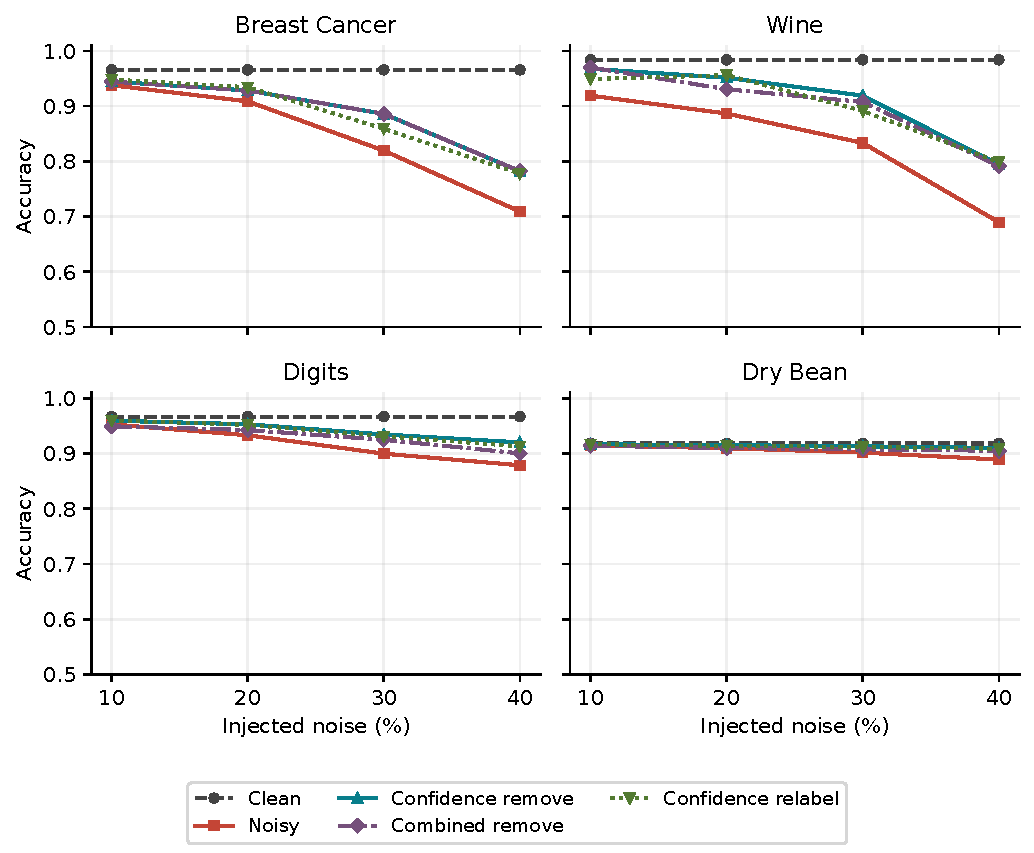
\includegraphics[width=\linewidth]{accuracy_symmetric.pdf}
\caption{Accuracy under symmetric corruption. Each point averages three
models and four seeds within a dataset. Selected methods are shown for
legibility; all methods appear in Table~\ref{tab:overall}. Lines connect the
four evaluated rates and do not represent fitted continuous trends.}
\label{fig:symmetric}
\end{figure}
\begin{figure}[htbp]
\centering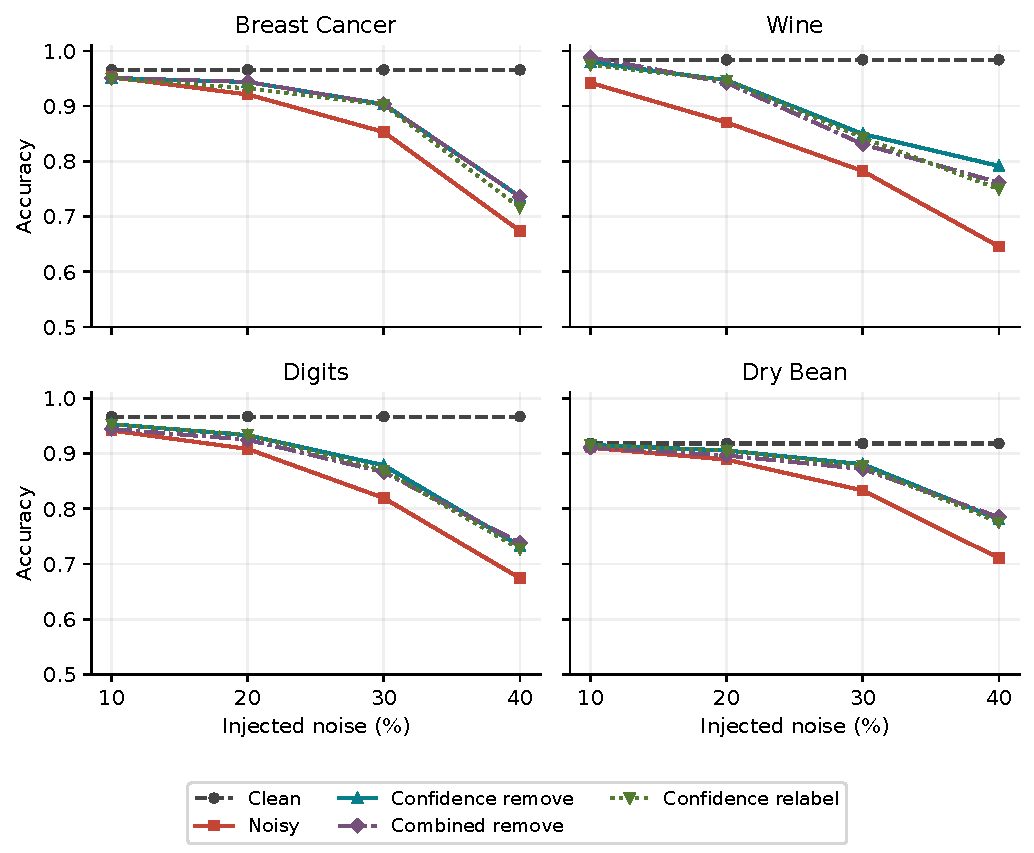
\includegraphics[width=\linewidth]{accuracy_class_dependent.pdf}
\caption{Accuracy under cyclic class-dependent corruption, aggregated as in
Fig.~\ref{fig:symmetric}. High-rate cyclic corruption is particularly damaging
on the multiclass tasks.}
\label{fig:cyclic}
\end{figure}

\subsection{Variation across Model Families}
Table~\ref{tab:models} reports dataset--model means across rates, mechanisms,
and seeds. RF has the strongest mean noisy-label accuracy on Wine and Digits;
LR has the strongest on Dry Bean. HGB has lower mean noisy accuracy than both
other models on each of the four datasets. This is evidence about the fixed
settings used here, not about optimally tuned boosting in general.
For Wine, HGB rises from 0.7439 to 0.8429 after confidence removal but remains
below the cleaned RF value of 0.9418.

\reporttable{models}{Mean test accuracy by dataset and classifier.}{tab:models}
{LR: logistic regression; RF: random forest; HGB: histogram gradient boosting.
Each cell averages two noise types, four rates, and four seeds. ``Conf.'' and
``Comb.'' denote confidence and combined scoring; rem./rel. denote removal/relabeling.}

Removal is not always preferable to relabeling. On Digits with RF, confidence
relabeling reaches 0.9370 versus 0.9330 for removal. On Dry Bean with HGB,
the corresponding means are nearly tied. A global average therefore does
not justify selecting one action blindly for every model--dataset pair.

\section{RQ2: Detection of Injected Errors}
Table~\ref{tab:detection} counts each detector once per experimental combination,
not once for both removal and relabeling. Confidence has the highest average
detection F1, 0.8072, followed by combined, 0.7504, disagreement, 0.6827, and
margin, 0.2425. Because the selected fraction closely matches the injected
fraction, precision and recall are nearly equal; this is partly a design
property rather than independent evidence from two unrelated criteria.

\reporttable{detection}{Injected-label-error detection, averaged over 384 combinations per detector.}{tab:detection}
{Detection is evaluated on training rows. Removal and relabeling share each
detector's mask and are not double-counted.}

\begin{figure}[htbp]
\centering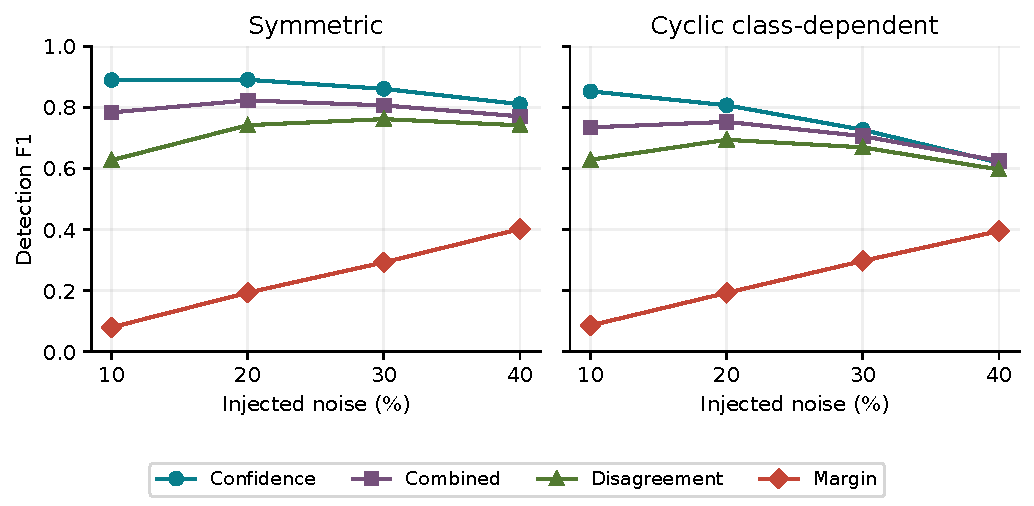
\includegraphics[width=\linewidth]{detection.pdf}
\caption{Detection F1 by nominal rate and corruption mechanism. Each point
averages the four datasets, three models, and four seeds. No test labels are
used to compute a suspiciousness score.}
\label{fig:detection}
\end{figure}

Margin-only selection behaves differently from confidence selection.
A confidently wrong observed label can receive a low margin score when the
model strongly predicts another class. Conversely, a correctly labeled but
ambiguous example can receive a high margin score. The poor detection and
downstream outcomes are consistent with this mismatch between uncertainty
and label error. This is a mechanism-based interpretation of the scores,
not a causal experiment isolating boundary examples.

\section{RQ3: Effects of Cleaning and Relabeling}
Figure~\ref{fig:gains} shows the paired accuracy gain within each dataset.
Confidence removal improves all four dataset-level averages, from 2.24
points on Dry Bean to 7.87 points on Wine. Margin removal reduces all four
averages, from 4.14 points on Dry Bean to 7.12 points on Digits. This pattern
is not merely the result of pooling the largest dataset with smaller ones:
datasets receive equal weight and their separate effects are visible.

\begin{figure}[htbp]
\centering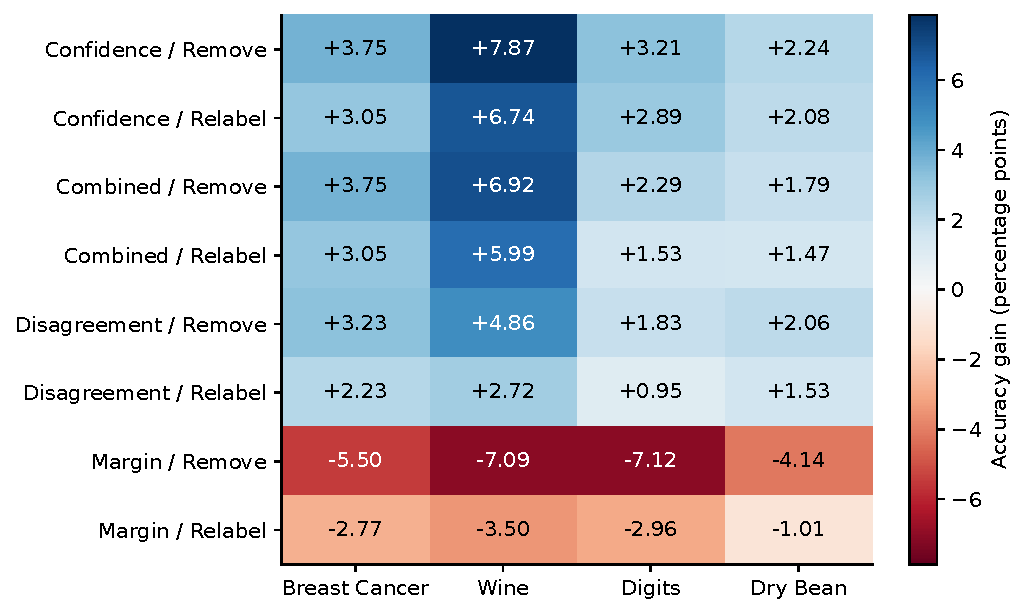
\includegraphics[width=\linewidth]{dataset_gains.pdf}
\caption{Paired accuracy gains over noisy training, in percentage points.
Every cell averages 24 settings and four seeds for one dataset. Numeric
annotations preserve interpretation without color.}
\label{fig:gains}
\end{figure}

Table~\ref{tab:inference} reports both effect size and the limits of inference.
Confidence removal improves 94.8\% of the 96 seed-averaged settings. This is
not the same as its proportion of individually improved seed runs: aggregation
reduces some seed variability before a setting is counted as a win.
The confidence-removal exploratory interval is entirely positive, yet the
exact two-sided $p$-value is 0.125 and its Holm-adjusted value is 1.000.
There is no contradiction: the bootstrap percentile interval and discrete
exact test answer the uncertainty question differently with very sparse
dataset-level evidence. The interval must not be used to claim significance.

\reporttable{inference}{Paired accuracy effects and exploratory dataset-level inference.}{tab:inference}
{Gain and interval endpoints are percentage points. Intervals resample four
dataset means. Win rates use 96 seed-averaged settings. $p_H$ is Holm-adjusted
within the eight accuracy comparisons. None is significant at 0.05.}

\subsection{Does the Combined Score Help?}
The direct comparison in Table~\ref{tab:ablation} gives combined removal an
average deficit of 0.58 accuracy points relative to confidence removal;
combined relabeling has a deficit of 0.68 points. Combined scoring exceeds
disagreement and margin on the grand mean, but does not beat the best simple
component. All reported adjusted comparisons remain nonsignificant.

\reporttable{ablation}{Combined scoring minus each component detector under the same action.}{tab:ablation}
{Positive gain favors combined. Each comparison uses matched
dataset--model--noise--rate--seed observations; inference uses four dataset
means. Holm adjustment covers the six accuracy comparisons.}

Breast Cancer's combined and confidence downstream results coincide in the
aggregate, as the binary ranking analysis predicts. For each of the three
multiclass datasets, confidence has a larger mean gain for both actions.
The combination can shift highly uncertain examples upward without providing
additional evidence that their observed labels are wrong. A different weight
choice might behave differently, but choosing it after inspecting these
test results would require a new, independently evaluated selection procedure.
The present negative result should not be obscured by retrospective tuning.

\subsection{A Concrete Failure despite Good Detection}
The saved-model example uses Dry Bean, RF, symmetric 20\% noise, confidence
scoring, and seed 42. Table~\ref{tab:diagnostic} makes the failure case explicit.
Detection F1 is 0.9151, but removal and relabeling both reduce test accuracy
relative to the noisy baseline. They improve macro AUROC in this setting,
showing that probability ranking and hard-label accuracy can move in
different directions. The small differences do not support a separate
statistical conclusion from one seed.

\reporttable{diagnostic}{Illustrative saved-model setting: Dry Bean/RF/symmetric 20\%/seed 42.}{tab:diagnostic}
{Confidence is used for both cleaning actions. PR AUC is the trapezoidal area
under the micro-averaged precision--recall curve, not average precision.}

The noisy classifier's confusion matrix in Fig.~\ref{fig:confusion} identifies
where residual errors occur. Class IDs are defined in Chapter~4. This example
is a diagnostic illustration, not an unbiased choice of the best-performing
setting. The full matrix, rather than this single case, supports the aggregate
comparison. ROC and PR curves for the same saved classifier are provided in
Appendix~A.

\begin{figure}[htbp]
\centering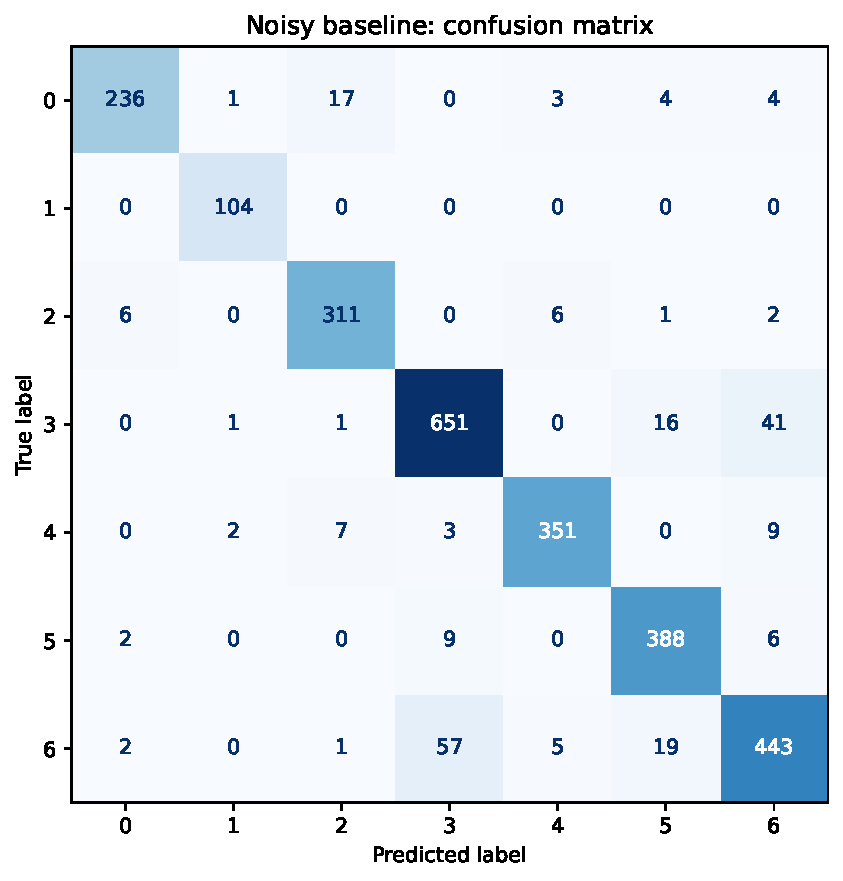
\includegraphics[width=.88\linewidth]{noisy_baseline_confusion_matrix.pdf}
\caption{Test confusion matrix for the illustrative noisy RF classifier.
Rows are reference classes and columns predicted classes. The test set has
2,709 examples and was not corrupted.}
\label{fig:confusion}
\end{figure}

\section{Threats to Validity}
\textbf{Internal validity.} Shared splits, training-only out-of-fold scoring,
pipeline-local scaling, exact-count corruption, and duplicate removal reduce
leakage risk. Saved checksums and re-execution provide evidence that the
tables correspond to the code. Nevertheless, testing cannot exclude every
implementation error. The same integer seed drives multiple random processes;
results use deterministic paired conditions rather than independently
randomized substreams. A future design could study sensitivity to separate
split, corruption, and estimator seeds.

\textbf{Construct validity.} The injected mask is an operational definition
of noise. It does not establish that the original labels are correct. The
cyclic transition is arbitrary in class-ID space, and the known-rate budget
is unavailable in many applications. Margin measures uncertainty, while
confidence combines possible label error with model misspecification.
The reserved validation data are unused; this avoids tuning leakage but
does not evaluate practical threshold selection.

\textbf{External validity.} Four numeric datasets, only one binary task,
and no real audited annotation errors limit generalization. Digits is
image-derived and the other datasets are relatively small. There are no
mixed categorical tables, deployment shifts, feature-noise experiments,
or calibrated estimates of label-error prevalence. No clinical or other
high-stakes use is supported by these experiments.
Random stratified partitions do not establish generalization to unseen
patients, writers, or collection sites; subject-group independence is not
evaluated by this benchmark.

\textbf{Comparative validity.} Only fixed estimator parameters and four
simple scores are compared. Confident learning, robust losses, stronger
tabular learners, instance-dependent corruption, and adaptive budgets remain
unmeasured. No runtime benchmark establishes that the proposed pipeline is
faster than alternatives. The combined score's modest engineering complexity
is not evidence of a new algorithmic contribution.

\textbf{Statistical validity.} The 3,840 rows share datasets, splits,
corruptions, and repeated references. They cannot be treated as independent
replicates. Four dataset means are insufficient for precise population-level
inference; the convenience sample also weakens generalization beyond the
observed tasks. Retrospective best-by-setting tables are descriptive only
and are not an evaluated model-selection policy.

\chapter{Conclusion and Future Work}
\section{Answers to the Research Questions}
\textbf{RQ1:} Training-label corruption reduces aggregate performance and
its effect depends strongly on dataset, model, and transition structure.
The mean clean-reference accuracy is \CleanAccuracy{}, compared with
\NoisyAccuracy{} for noisy training. High-rate cyclic corruption is
particularly damaging on Digits and Dry Bean. Fixed-default HGB is more
sensitive than the other evaluated families on the dataset-level means,
but this is not a conclusion about optimally tuned boosting.

\textbf{RQ2:} Out-of-fold confidence is the most effective of the four
evaluated detectors on average, with detection F1 of 0.8072. Combined
scoring follows at 0.7504. General uncertainty, measured by the top-two
probability margin, is a poor proxy for injected label errors in this design.
The shared out-of-fold matrix and common selection budget make the component
comparison directly interpretable.

\textbf{RQ3:} Confidence-based removal improves average test accuracy by
\ConfidenceRemoveGain{} percentage points and combined removal by
\CombinedRemoveGain{} points. Neither closes the full gap to clean training.
Relabeling helps on average for three detectors, but is not uniformly better
than removal. High detection quality does not guarantee a downstream accuracy
gain, as the saved Dry Bean example demonstrates. Margin-only cleaning is
harmful on all four dataset-level averages.

\section{Contribution Supported by the Evidence}
The project delivers a reproducible benchmark and a transparent evaluation of
a simple combined-score hypothesis. The hypothesis does not succeed against
confidence alone on the aggregate comparison. The binary analysis explains
why the combination often cannot change confidence's ranking; the multiclass
experiments show that changing the ranking does not necessarily improve it.
These results favor starting with a simple confidence baseline before adding
uncertainty terms, within the controlled setting tested here.

The release includes an auditable matrix, generated tables and figures,
illustrative saved models, tests, pinned dependencies, and an immutable
Git-LFS archive. This supports verification and extension of the experiment,
not a claim of universal method superiority. With four datasets, no exact
two-sided comparison can reach significance at 0.05. Conclusions remain
descriptive and exploratory.

\section{Priorities for Future Work}
The first priority is to remove the oracle-budget assumption. A future study
should choose thresholds or removal fractions using only training information
or a properly allocated validation set, then evaluate the complete selection
procedure on untouched test data. This would test whether the current gains
survive uncertainty about the actual noise prevalence.

Second, the comparison should add established label-quality methods such as
confident learning, alternative cyclic maps, and feature-dependent corruptions.
Real annotation-error datasets would distinguish injected-error recovery from
genuine data-quality improvement. Additional mixed-type tabular datasets
would broaden the empirical population and improve the resolution of
dataset-level inference.

Third, model and score choices should be evaluated under a prespecified tuning
protocol. Probability calibration, class-aware selection budgets, and
confidence-gated relabeling are reasonable hypotheses, but should not be
selected from the current test outcomes and presented as already validated.
Randomized tie handling and separately seeded random processes are additional
sensitivity checks. Finally, controlled runtime and memory measurements
would turn the qualitative term ``lightweight'' into a measured cost comparison.

\clearpage
\phantomsection
\addcontentsline{toc}{chapter}{References}
\bibliographystyle{IEEEtran}
\bibliography{report/references}
\appendix
\chapter{Reproducibility and Supplementary Diagnostics}
\section{Immutable Evidence}
The report is based on the code/results release at revision:
\begin{quote}\small\path{50f8995a014f4d68714cba7a4ea81e911c859374}\end{quote}
The original training revision is:
\begin{quote}\small\path{2d0dfbf34480bba5e602f165fd12dc0c3ef75ef8}\end{quote}
Later report commits do not
rewrite the historical training record.

The main result CSV contains 3,840 rows and has SHA-256
\begin{quote}\small\ttfamily
\path{2576804e3caadd3025ff95a9835729ced219fd38dce4ca30ee4a399727a61150}.
\end{quote}
The archive \path{releases/code-results-50f8995.tar.gz} has SHA-256
\begin{quote}\small\ttfamily
\path{73b15ce8a707f671f7d7102d8ac776d504a9786afda5d933f0a72e7363861e58}.
\end{quote}
It contains 264 source and artifact files, including the 181 items in the
frozen audit inventory. The source repository is
\url{https://github.com/Ovais09/csi6900-noisy-labels}. Git LFS stores the large
archive separately from the ordinary Git pointer. It must be fetched before
extracting the release. The archive must not be unpacked over an active
working tree, and untrusted serialized models must not be loaded.

\section{Artifact Map}
\begin{longtable}{>{\raggedright\arraybackslash}p{.38\linewidth}>{\raggedright\arraybackslash}p{.55\linewidth}}
\toprule
Artifact & Purpose \\
\midrule
\endhead
\path{configs/experiment_config.yaml} & Exact experimental grid. \\
\path{results/tables/main_experiment_results.csv} & Per-combination and per-condition metrics and counts. \\
\path{results/tables/summary_results.csv} & 960 rows aggregating the four seeds within settings. \\
\path{results/tables/analysis/} & Eight analysis tables, including paired cleaning and direct detector comparisons. \\
\path{results/models/} & Four RF models for one Dry Bean setting, not all models fitted by the benchmark. \\
\path{results/figures/} & 60 main and 13 diagnostic figures, each in PNG and PDF. \\
\path{results/logs/run_manifest.json} & Config, data, environment, result, and original training provenance. \\
\path{results/logs/release_manifest.json} & Artifact sizes and SHA-256 hashes. \\
\path{results/logs/final_audit.json} & Passing audit of that frozen inventory. \\
\path{report/generated/evidence.json} & Checksummed inputs used to generate report tables and figures. \\
\bottomrule
\end{longtable}

The report generator recomputes analysis tables from the exact CSV and checks
them against the frozen versions before producing LaTeX tables. Numeric
summary tables are not manually transcribed. Report-specific plots average
the same matrix; selected diagnostic PDFs are copied unchanged after hash
verification. Their source values and revision are recorded in the evidence
file. The IEEEtran BibTeX style produces the numbered bibliography.

\section{Build and Reproduction Commands}
The complete extraction and audit commands are in \path{releases/README.md}.
The following commands assume the Git-LFS archive has been verified and
restored to an empty \path{releases/restored/} directory:
\begin{lstlisting}
python scripts/make_report_assets.py --release-root releases/restored
docker build -f report/Dockerfile -t csi6900-report .
docker run --rm --network none -v "$PWD:/work" csi6900-report
\end{lstlisting}
The last command runs pdfLaTeX and BibTeX through latexmk and writes
\path{report/build/main.pdf}. Building from the already committed report
assets does not require model training or downloading datasets. A full
benchmark rerun uses the archived configuration and pipeline in its own
checkout; it should not overwrite the frozen evidence used by this report.

\section{Preparation and Review}
AI assistance was used during software implementation, testing, analysis
support, and manuscript preparation. The numerical evidence is tied to the
saved experiment artifacts, not generated as illustrative data. Source
verification and software checks do not replace the author's responsibility
to understand the methods, review the conclusions, and comply with the
supervisor's and institution's requirements for assistance and disclosure.

\section{Supplementary Macro F1 and Curves}
Figure~\ref{fig:f1} provides the macro-F1 counterpart of the cyclic accuracy
plot. Figures~\ref{fig:roc} and \ref{fig:pr} concern only the saved noisy RF
classifier from the Dry Bean diagnostic setting. Their smooth ranking
summaries should not be interpreted as proof that cleaning improves the
hard-label predictions in that setting.

\begin{figure}[htbp]
\centering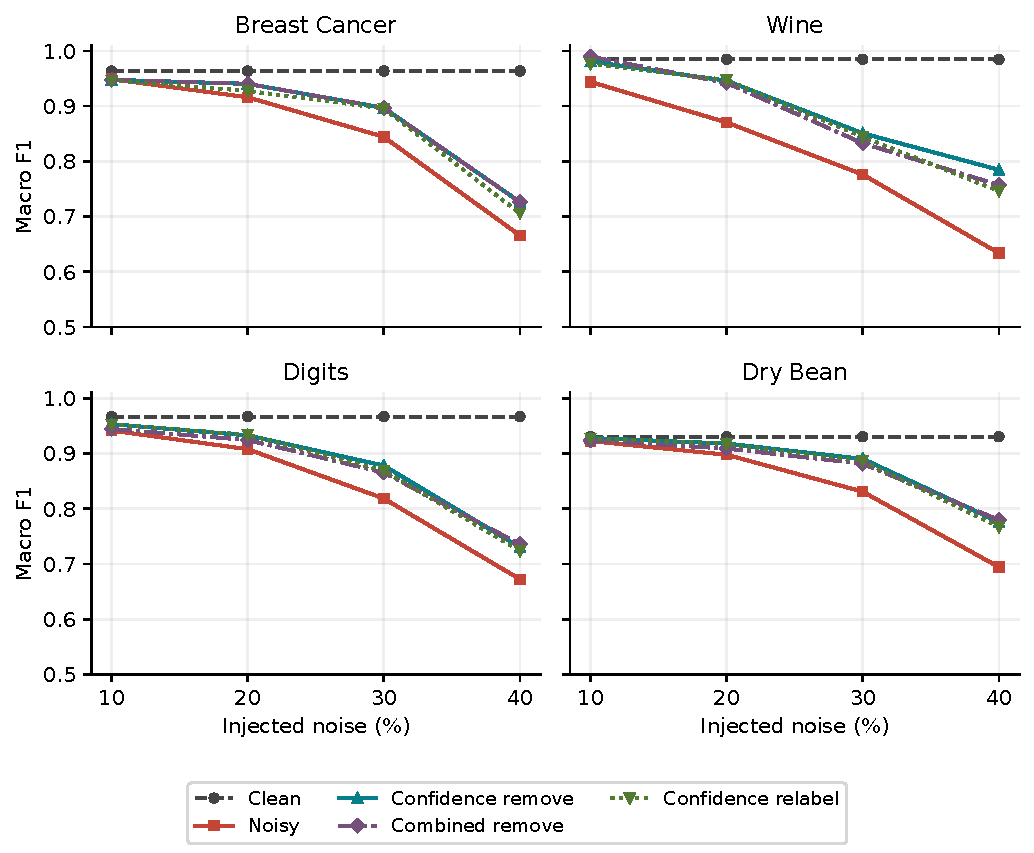
\includegraphics[width=\linewidth]{f1_macro_class_dependent.pdf}
\caption{Macro F1 under cyclic class-dependent corruption. Each point averages
three models and four seeds within a dataset. The plotted methods and rates
match the main accuracy comparison.}
\label{fig:f1}
\end{figure}
\begin{figure}[htbp]
\centering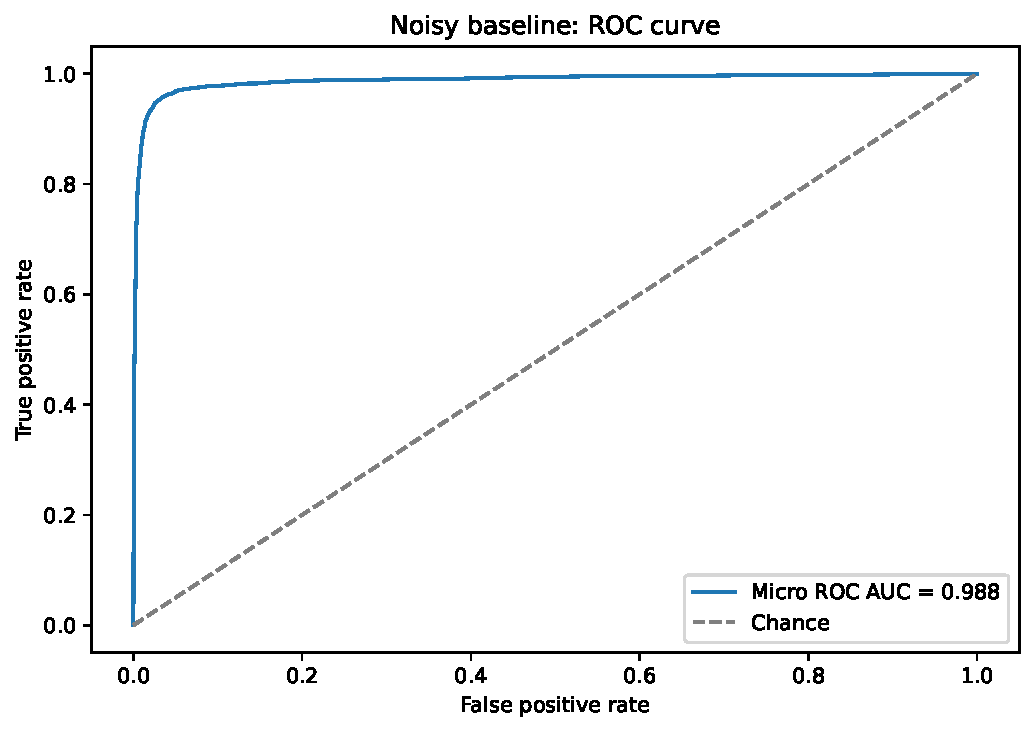
\includegraphics[width=.9\linewidth]{noisy_baseline_roc_curve.pdf}
\caption{Micro-averaged ROC curve for the noisy Dry Bean RF classifier,
symmetric 20\% corruption and seed 42. Micro ROC AUC is approximately 0.9878;
the main metric for this model is macro one-vs-rest AUROC, approximately 0.9874.}
\label{fig:roc}
\end{figure}
\begin{figure}[htbp]
\centering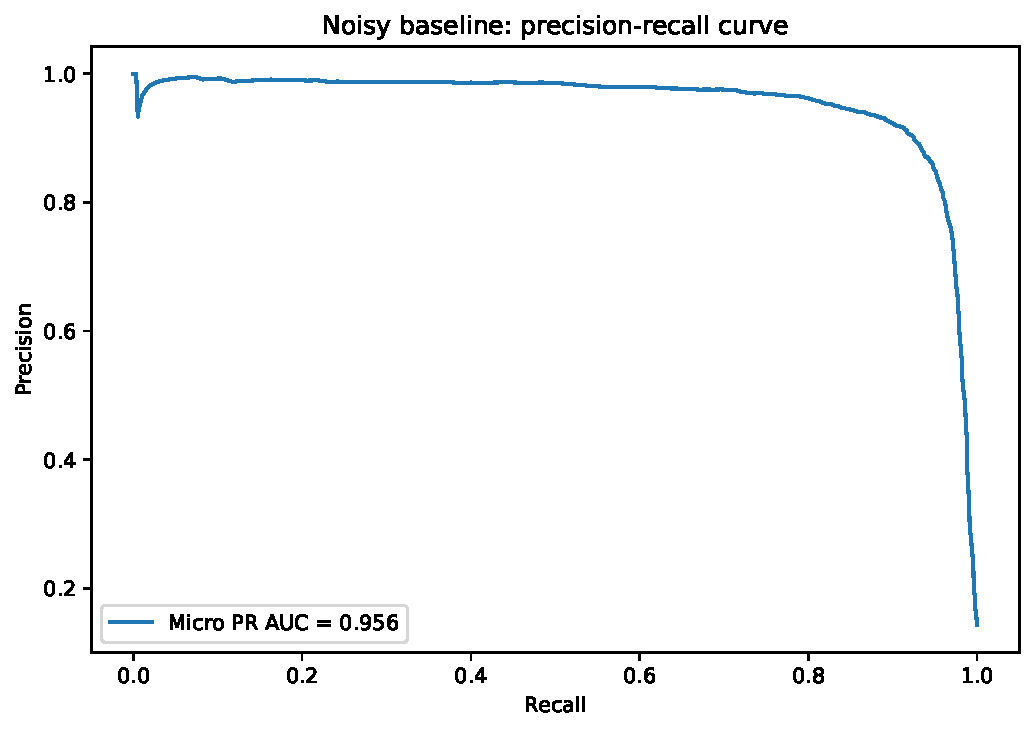
\includegraphics[width=.9\linewidth]{noisy_baseline_precision_recall_curve.pdf}
\caption{Micro-averaged precision--recall curve for the same noisy classifier.
Trapezoidal PR AUC is approximately 0.9558. This is not average precision.}
\label{fig:pr}
\end{figure}

\end{document}
